W tym rozdziale przedstawiono przeprowadzone badania, sposób ich przeprowadzenia, przedstawiono sprzęt, na którym przeprowadzono badania.
\section{Opis komputera}
Wszystkie testy oraz badania zostały przeprowadzone na maszynie zaprezentowanej w tabeli \ref{tab:machine}. W tabeli wymieniono tylko znaczące elementy, tzn. procesor, pamięć RAM oraz jej szybkość, dysk twardy, jego prędkość obrotową oraz typ. Wszystkie te podzespoły mogą wpływać na czas trwania elementów działania aplikacji. Ze względu na jednowątkowość aplikacji, nie podaje się ilości wątków.
\begin{table}[H]
    \centering
    \begin{tabular}{|l|l|}
        \hline
        Procesor       & Intel Core-i5 8600 @ 3.10 GHz          \\ \hline
        Pamięć RAM     & 16GB DDR4 @ 3200 MHz \\ \hline
        Typ dysku twardego           & HDD              \\ \hline
        Dysk twardy         & Toshiba HDWD110              \\ \hline
        Prędkość obrotowa         & 7200 obr./min              \\ \hline
    \end{tabular}
    \caption{Spis części}
    \label{tab:machine}
\end{table}
Wszystkie pliki aplikacji zostały umieszczone na dysku HDD. Instancja baza danych znajduje się na dysku instalacyjnym, który jest rodzaju SSD.
\section{Parametry danych wejściowych}
\label{sec:entryparamters}
30 pomiarów, 48 plików
\section{Przeprowadzone pomiary}
W tym podrozdziale zostaną zaprezentowane otrzymane wyniki, których format zaprezentowano w sekcji \ref{ssec:exitdata}. Dodatkowo do każdego wyniku została przygotowana krótka analiza wraz z zaprezentowaniem dopełniających parametrów wyników, umożliwiających lepszą interpretację rezultatów. Rozpoczęto od analizy możliwych rodzajów kalibracji danych wejściowych, wraz z pomiarem czasu. Kolejnym elementem jest ukazanie wpływu parametrów wewnętrznych algorytmów na wyniki końcowe. Trzecia sekcja porównuje czasy trwania algorytmów, wraz z analizą przyczyn różnic czasowych. Następna sekcja opisuje wyniki obciążenia pamięciowego przez zaimplementowane algorytmy wykrywania fiksacji, jak również opisuje najbardziej obciążające metody. W przedostatnim podrozdziale zanalizowano metody wprowadzania danych wejściowych do aplikacji. Ostatnia analiza dotyczy dokładności algorytmu uczenia maszynowego oraz porównania wynikowych punktów wszystkich trzech algorytmów przedstawionych w sekcji \ref{ssec:algorithms}.
\subsection{Analiza kalibracji danych}
\label{ssec:calibration}
Wykorzystane rozwiązanie dotyczące kalibracji punktów zostało opisane w sekcji \ref{ssec:calibrationtheory}. Zdecydowano się na wykorzystanie rozwiązania liniowego, pomimo nieliniowości punktów, ze względu na problemy z implementacją algorytmów wielomianowych, z wykorzystaniem metod \textbf{np.polyfit} oraz \textbf{np.polyval}, których zadaniem jest utworzenie takiej funkcji wielomianowej. Dodatkowo brak doświadczenia w pracy z takimi rozwiązaniami mógł przyczynić się do niepowodzenia. Przykład takiej błędnej kalibracji zaprezentowano na rysunku \ref{fig:error_cal}.
\begin{figure}[H]
    \centering
    \captionsetup{justification=centering,margin=2cm}
    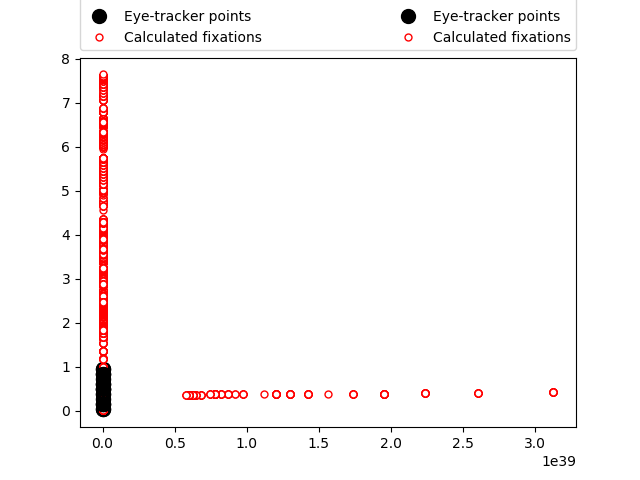
\includegraphics[width=\linewidth]{resources/error_cal.png}
    \caption{Błędnie skalibrowany element}
    \label{fig:error_cal}
\end{figure}
W tabeli \ref{tab:calibration} zaprezentowano pomiar czasu kalibracji wszystkich danych dla każdego pliku. Czas ten zaprezentowano w sekundach. Dodatkowymi obliczonymi parametrami są suma wszystkich kalibracji: 97,234375 sekund, średni czas trwania kalibracji:	2,02572 sekund, odchylenie standardowe: 0,07297 sekund, mediana wyników: 2,015625 oraz wartości maksymalne i minimalne - odpowiednio 2,203125 sekund i 1,90625
\begin{longtable}{|l|r|}
    \hline
    \multicolumn{1}{|c|}{\textbf{Plik wejściowy}} & \multicolumn{1}{c|}{\textbf{Łączny czas kalibracji}} \\ \hline
    \endfirsthead
    %
    \multicolumn{2}{c}%
    {{\bfseries Kontynuacja tabeli \thetable\ z poprzedniej strony}} \\
    \hline
    \multicolumn{1}{|c|}{\textbf{Plik wejściowy}} & \multicolumn{1}{c|}{\textbf{Łączny czas kalibracji}} \\ \hline
    \endhead
    %
    1\_01\_1311201811.cal & 2,140625 \\ \hline
    1\_02\_1310301856.cal & 2,0625 \\ \hline
    1\_03\_1310301904.cal & 1,953125 \\ \hline
    1\_04\_1310301810.cal & 1,96875 \\ \hline
    1\_05\_1310301817.cal & 2,078125 \\ \hline
    1\_06\_1310301837.cal & 1,921875 \\ \hline
    1\_12\_1310301901.cal & 1,953125 \\ \hline
    1\_14\_1310301912.cal & 1,953125 \\ \hline
    1\_15\_1310301840.cal & 2,03125 \\ \hline
    1\_16\_1310301844.cal & 2,1875 \\ \hline
    1\_17\_1310301825.cal & 2,125 \\ \hline
    1\_20\_1310301822.cal & 1,984375 \\ \hline
    1\_21\_1310301833.cal & 1,90625 \\ \hline
    1\_22\_1310301908.cal & 2,0625 \\ \hline
    1\_23\_1310301722.cal & 2,03125 \\ \hline
    1\_24\_1311201804.cal & 1,984375 \\ \hline
    1\_25\_1311201806.cal & 1,984375 \\ \hline
    1\_26\_1311201835.cal & 2,0625 \\ \hline
    1\_27\_1311201823.cal & 1,90625 \\ \hline
    1\_28\_1310301813.cal & 2,015625 \\ \hline
    1\_29\_1310301914.cal & 1,984375 \\ \hline
    1\_31\_1310301807.cal & 2,09375 \\ \hline
    1\_32\_1310301831.cal & 2 \\ \hline
    1\_34\_1310301804.cal & 2,171875 \\ \hline
    3\_01\_1401151823.cal & 2,03125 \\ \hline
    3\_02\_1401151905.cal & 2,0625 \\ \hline
    3\_03\_1401151858.cal & 1,953125 \\ \hline
    3\_04\_1401151803.cal & 1,96875 \\ \hline
    3\_05\_1401151752.cal & 2,15625 \\ \hline
    3\_06\_1311201818.cal & 2,140625 \\ \hline
    3\_12\_1401151843.cal & 2,046875 \\ \hline
    3\_14\_1401151837.cal & 1,921875 \\ \hline
    3\_15\_1401151641.cal & 1,96875 \\ \hline
    3\_16\_1401151847.cal & 2,03125 \\ \hline
    3\_17\_1401151814.cal & 1,9375 \\ \hline
    3\_20\_1401151759.cal & 2 \\ \hline
    3\_21\_1401151911.cal & 2 \\ \hline
    3\_22\_1401151828.cal & 1,984375 \\ \hline
    3\_23\_1401151854.cal & 2 \\ \hline
    3\_24\_1401151840.cal & 2,015625 \\ \hline
    3\_25\_1401151908.cal & 2,203125 \\ \hline
    3\_26\_1401151826.cal & 2,03125 \\ \hline
    3\_27\_1401151811.cal & 2 \\ \hline
    3\_28\_1401151747.cal & 2,0625 \\ \hline
    3\_29\_1401151833.cal & 2,0625 \\ \hline
    3\_31\_1401151755.cal & 2,078125 \\ \hline
    3\_32\_1401151808.cal & 2,046875 \\ \hline
    3\_34\_1401151805.cal & 1,96875 \\ \hline
    \caption{Pomiar czasów kalibracji}
    \label{tab:calibration}\\
    \end{longtable}
Jak można zauważyć na wynikach, kalibracja pomimo wykorzystania zewnętrznej biblioteki oraz operacji na tablicach, nie wymaga zbytniego wkładu czasowego w jej realizację. Odchylenie mieszczące się w granicy 2-3\% dla całości algorytmu zawiera się w dopuszczalnej granicy, prawdopodobnie jest ono spowodowane różnicą w ilości danych dostarczanych. Algorytm jest wydajny ze względu na czas około dwóch sekund dla całego pliku.
\subsection{Analiza wpływu parametrów algorytmów}
\label{ssec:queryparameters}
\subsection{Porównanie czasów trwania algorytmów}
\label{ssec:times}
\subsection{Analiza obciążenia pamięci}
\label{ssec:memory}
\newpage
\subsection{Analiza metod wprowadzania danych wejściowych}
\label{ssec:entrydata}
Celem poniższej sekcji jest prezentacja otrzymanych wyników pomiaru czasów pobrania danych wejściowych oraz ich konwersji na format czytelny dla aplikacji. Pierwsza kolumna w tabelach \ref{tab:fileimport} i \ref{tab:importdb} zawiera nazwę pliku, a w drugiej kolumnie znajdziemy wartości wykonanego pomiaru podane w sekundach.\par
W tabeli \ref{tab:fileimport} zaprezentowano wynik pomiaru importu danych oraz konwersji plików na format czytelny dla aplikacji pomiarowej. Obliczono także następujące wartości: łączny czas trwania importu danych wynosi 65,673 sekund, średni czas wynosi 1,3681875, odchylenie standardowe równa się 0,03755 w przybliżeniu do 5 miejsc po przecinku, a mediana wynosi 1,359 sekundy. Elementy maksymalne i minimalne wynoszą odpowiednio: 1,438 i
1,297 sekundy. Zgodnie z wartościami pokazanymi w sekcji \ref{sec:entryparamters}, oznacza to iż średnio 65734 elementów jest przetwarzanych na sekundę.
\begin{longtable}{|l|l|}
    \hline
    \multicolumn{1}{|c|}{\textbf{Plik wejściowy}} & \multicolumn{1}{c|}{\textbf{Czas wczytywania i konwersji}} \\ \hline
    \endfirsthead
    %
    \multicolumn{2}{c}%
    {{\bfseries Kontynuacja tabeli \thetable\ z poprzedniej strony}} \\
    \hline
    \multicolumn{1}{|c|}{\textbf{Plik wejściowy}} & \multicolumn{1}{c|}{\textbf{Czas wczytywania i konwersji}} \\ \hline
    \endhead
    %
    1\_01\_1311201811.cal & 1.344 \\ \hline
    1\_02\_1310301856.cal & 1.328 \\ \hline
    1\_03\_1310301904.cal & 1.375 \\ \hline
    1\_04\_1310301810.cal & 1.312 \\ \hline
    1\_05\_1310301817.cal & 1.344 \\ \hline
    1\_06\_1310301837.cal & 1.328 \\ \hline
    1\_12\_1310301901.cal & 1.297 \\ \hline
    1\_14\_1310301912.cal & 1.297 \\ \hline
    1\_15\_1310301840.cal & 1.312 \\ \hline
    1\_16\_1310301844.cal & 1.359 \\ \hline
    1\_17\_1310301825.cal & 1.391 \\ \hline
    1\_20\_1310301822.cal & 1.438 \\ \hline
    1\_21\_1310301833.cal & 1.359 \\ \hline
    1\_22\_1310301908.cal & 1.359 \\ \hline
    1\_23\_1310301722.cal & 1.344 \\ \hline
    1\_24\_1311201804.cal & 1.328 \\ \hline
    1\_25\_1311201806.cal & 1.344 \\ \hline
    1\_26\_1311201835.cal & 1.344 \\ \hline
    1\_27\_1311201823.cal & 1.359 \\ \hline
    1\_28\_1310301813.cal & 1.391 \\ \hline
    1\_29\_1310301914.cal & 1.375 \\ \hline
    1\_31\_1310301807.cal & 1.438 \\ \hline
    1\_32\_1310301831.cal & 1.406 \\ \hline
    1\_34\_1310301804.cal & 1.391 \\ \hline
    3\_01\_1401151823.cal & 1.406 \\ \hline
    3\_02\_1401151905.cal & 1.438 \\ \hline
    3\_03\_1401151858.cal & 1.344 \\ \hline
    3\_04\_1401151803.cal & 1.344 \\ \hline
    3\_05\_1401151752.cal & 1.359 \\ \hline
    3\_06\_1311201818.cal & 1.406 \\ \hline
    3\_12\_1401151843.cal & 1.391 \\ \hline
    3\_14\_1401151837.cal & 1.375 \\ \hline
    3\_15\_1401151641.cal & 1.312 \\ \hline
    3\_16\_1401151847.cal & 1.391 \\ \hline
    3\_17\_1401151814.cal & 1.375 \\ \hline
    3\_20\_1401151759.cal & 1.359 \\ \hline
    3\_21\_1401151911.cal & 1.344 \\ \hline
    3\_22\_1401151828.cal & 1.422 \\ \hline
    3\_23\_1401151854.cal & 1.344 \\ \hline
    3\_24\_1401151840.cal & 1.344 \\ \hline
    3\_25\_1401151908.cal & 1.406 \\ \hline
    3\_26\_1401151826.cal & 1.422 \\ \hline
    3\_27\_1401151811.cal & 1.406 \\ \hline
    3\_28\_1401151747.cal & 1.359 \\ \hline
    3\_29\_1401151833.cal & 1.344 \\ \hline
    3\_31\_1401151755.cal & 1.375 \\ \hline
    3\_32\_1401151808.cal & 1.422 \\ \hline
    3\_34\_1401151805.cal & 1.422 \\ \hline
    \caption{Czas wczytywania plików oraz konwersji z pliku .cal}
    \label{tab:fileimport}
\end{longtable}
Tabela \ref{tab:importdb} przedstawia odpowiadające wyniki dla pobierania elementów z bazy danych. Łączny czas tej operacji dla wszystkich 48 plików wynosi 118,395 sekund. Średni czas trwania równa się 2,4665625 s, odchylenie standardowe osiąga wartość 0,06259 w przybliżeniu do 5 miejsca po przecinku. Mediana wynosi 2,453 sekundy, wartość maksymalna 2,594 sekundy, a minimalna 2,344. Prędkość wykonywania operacji wynosi około 36488 elementów na sekundę.
\begin{longtable}{|l|l|}
    \hline
    \multicolumn{1}{|c|}{\textbf{Plik wejściowy}} & \multicolumn{1}{c|}{\textbf{Czas importu i konwersji}} \\ \hline
    \endfirsthead
    %
    \multicolumn{2}{c}%
    {{\bfseries Kontynuacja tabeli \thetable\ z poprzedniej strony}} \\
    \hline
    \multicolumn{1}{|c|}{\textbf{Plik wejściowy}} & \multicolumn{1}{c|}{\textbf{Czas importu i konwersji}} \\ \hline
    \endhead
    %
    1\_01\_1311201811.cal & 2.438 \\ \hline
    1\_02\_1310301856.cal & 2.422 \\ \hline
    1\_03\_1310301904.cal & 2.344 \\ \hline
    1\_04\_1310301810.cal & 2.391 \\ \hline
    1\_05\_1310301817.cal & 2.406 \\ \hline
    1\_06\_1310301837.cal & 2.375 \\ \hline
    1\_12\_1310301901.cal & 2.359 \\ \hline
    1\_14\_1310301912.cal & 2.344 \\ \hline
    1\_15\_1310301840.cal & 2.359 \\ \hline
    1\_16\_1310301844.cal & 2.547 \\ \hline
    1\_17\_1310301825.cal & 2.594 \\ \hline
    1\_20\_1310301822.cal & 2.547 \\ \hline
    1\_21\_1310301833.cal & 2.438 \\ \hline
    1\_22\_1310301908.cal & 2.516 \\ \hline
    1\_23\_1310301722.cal & 2.422 \\ \hline
    1\_24\_1311201804.cal & 2.391 \\ \hline
    1\_25\_1311201806.cal & 2.422 \\ \hline
    1\_26\_1311201835.cal & 2.469 \\ \hline
    1\_27\_1311201823.cal & 2.469 \\ \hline
    1\_28\_1310301813.cal & 2.438 \\ \hline
    1\_29\_1310301914.cal & 2.562 \\ \hline
    1\_31\_1310301807.cal & 2.562 \\ \hline
    1\_32\_1310301831.cal & 2.547 \\ \hline
    1\_34\_1310301804.cal & 2.531 \\ \hline
    3\_01\_1401151823.cal & 2.500 \\ \hline
    3\_02\_1401151905.cal & 2.422 \\ \hline
    3\_03\_1401151858.cal & 2.453 \\ \hline
    3\_04\_1401151803.cal & 2.422 \\ \hline
    3\_05\_1401151752.cal & 2.531 \\ \hline
    3\_06\_1311201818.cal & 2.516 \\ \hline
    3\_12\_1401151843.cal & 2.453 \\ \hline
    3\_14\_1401151837.cal & 2.453 \\ \hline
    3\_15\_1401151641.cal & 2.438 \\ \hline
    3\_16\_1401151847.cal & 2.516 \\ \hline
    3\_17\_1401151814.cal & 2.500 \\ \hline
    3\_20\_1401151759.cal & 2.453 \\ \hline
    3\_21\_1401151911.cal & 2.500 \\ \hline
    3\_22\_1401151828.cal & 2.438 \\ \hline
    3\_23\_1401151854.cal & 2.469 \\ \hline
    3\_24\_1401151840.cal & 2.438 \\ \hline
    3\_25\_1401151908.cal & 2.500 \\ \hline
    3\_26\_1401151826.cal & 2.438 \\ \hline
    3\_27\_1401151811.cal & 2.469 \\ \hline
    3\_28\_1401151747.cal & 2.547 \\ \hline
    3\_29\_1401151833.cal & 2.453 \\ \hline
    3\_31\_1401151755.cal & 2.500 \\ \hline
    3\_32\_1401151808.cal & 2.562 \\ \hline
    3\_34\_1401151805.cal & 2.531 \\ \hline
    \caption{Czas importu danych oraz konwersji z bazy danych}
    \label{tab:importdb}\\
\end{longtable}
Jak można zauważyć na powyższych wynikach, czas połączenia z bazą danych wynosi około sekundę dłużej niż przy połączeniu lokalnym. Obliczone wartości odchylenia standardowego przy tych metodach pobierania danych wskazują na to iż są one dość stabilne, gdyż ich odchylenie nie przekracza wartości 0,1 s, co dla operacji na takiej ilości danych nie przeszkadza w szybkiej analizie. Pomimo umieszczenia bazy danych na dysku SSD, czasy odczytu danych nie poprawiły się. Po umieszczeniu timera pomiędzy metodami inicjalizującymi połączenie stwierdzono iż zajmuje ono około 0,5 sekundy.
\par
W tabeli \ref{tab:insertdb} zaprezentowano wyniki pomiaru operacji importu danych do bazy danych. Zostało to wykonane celem weryfikacji wydajności bazy danych. Łączny czas operacji dla wszystkich plików wyniósł 180,432 sekundy, średnia otrzymana wartość to 3,759 sekund, 
odchylenie standardowe 0,74628 sekund, mediana 3,562 sekund, maksimum prawie 7 sekund a minimum 3,4 sekundy.
\begin{longtable}{|l|r|}
    \hline
    \multicolumn{1}{|c|}{\textbf{Plik wejściowy}} & \multicolumn{1}{c|}{\textbf{Czas importu danych do bazy danych}} \\ \hline
    \endfirsthead
    %
    \multicolumn{2}{c}%
    {{\bfseries Kontynuacja tabeli \thetable\ z poprzedniej strony}} \\
    \hline
    \multicolumn{1}{|c|}{\textbf{Plik wejściowy}} & \multicolumn{1}{c|}{\textbf{Czas importu danych do bazy danych}} \\ \hline
    \endhead
    %
    1\_01\_1311201811.cal & 3,484 \\ \hline
    1\_02\_1310301856.cal & 3,406 \\ \hline
    1\_03\_1310301904.cal & 3,484 \\ \hline
    1\_04\_1310301810.cal & 3,5 \\ \hline
    1\_05\_1310301817.cal & 3,453 \\ \hline
    1\_06\_1310301837.cal & 3,438 \\ \hline
    1\_12\_1310301901.cal & 6,734 \\ \hline
    1\_14\_1310301912.cal & 3,453 \\ \hline
    1\_15\_1310301840.cal & 3,453 \\ \hline
    1\_16\_1310301844.cal & 3,672 \\ \hline
    1\_17\_1310301825.cal & 3,828 \\ \hline
    1\_20\_1310301822.cal & 3,625 \\ \hline
    1\_21\_1310301833.cal & 3,516 \\ \hline
    1\_22\_1310301908.cal & 3,562 \\ \hline
    1\_23\_1310301722.cal & 3,484 \\ \hline
    1\_24\_1311201804.cal & 3,438 \\ \hline
    1\_25\_1311201806.cal & 6,812 \\ \hline
    1\_26\_1311201835.cal & 3,484 \\ \hline
    1\_27\_1311201823.cal & 3,672 \\ \hline
    1\_28\_1310301813.cal & 3,609 \\ \hline
    1\_29\_1310301914.cal & 6,312 \\ \hline
    1\_31\_1310301807.cal & 3,703 \\ \hline
    1\_32\_1310301831.cal & 3,656 \\ \hline
    1\_34\_1310301804.cal & 3,609 \\ \hline
    3\_01\_1401151823.cal & 3,562 \\ \hline
    3\_02\_1401151905.cal & 3,656 \\ \hline
    3\_03\_1401151858.cal & 3,453 \\ \hline
    3\_04\_1401151803.cal & 3,531 \\ \hline
    3\_05\_1401151752.cal & 3,547 \\ \hline
    3\_06\_1311201818.cal & 3,688 \\ \hline
    3\_12\_1401151843.cal & 3,609 \\ \hline
    3\_14\_1401151837.cal & 3,516 \\ \hline
    3\_15\_1401151641.cal & 3,516 \\ \hline
    3\_16\_1401151847.cal & 3,531 \\ \hline
    3\_17\_1401151814.cal & 3,547 \\ \hline
    3\_20\_1401151759.cal & 3,516 \\ \hline
    3\_21\_1401151911.cal & 3,594 \\ \hline
    3\_22\_1401151828.cal & 3,531 \\ \hline
    3\_23\_1401151854.cal & 3,625 \\ \hline
    3\_24\_1401151840.cal & 3,5 \\ \hline
    3\_25\_1401151908.cal & 3,734 \\ \hline
    3\_26\_1401151826.cal & 3,562 \\ \hline
    3\_27\_1401151811.cal & 3,547 \\ \hline
    3\_28\_1401151747.cal & 3,734 \\ \hline
    3\_29\_1401151833.cal & 3,562 \\ \hline
    3\_31\_1401151755.cal & 3,594 \\ \hline
    3\_32\_1401151808.cal & 3,734 \\ \hline
    3\_34\_1401151805.cal & 3,656 \\ \hline
    \caption{Pomiar czasu umieszczania elementów w bazie danych}
    \label{tab:insertdb}\\
\end{longtable}
Zastanawiającym wynikiem jest wynik 7 sekund przy zapisie do bazy danych, po weryfikacji prawdopodobną przyczyną takich pomiarów jest chwilowa niedyspozycyjność serwera do wykonywania operacji, jednak, jako iż tylko 2 operacje osiągnęły taki wynik, może to być też wynikiem przypadku, bo nie znaleziono żadnych anomalii przeszukując te dwa pliki.\\
Łączny średni czas operacji na bazie danych wynosi około 6,22 sekund, co dla ilości danych zaprezentowanych w sekcji \ref{sec:entryparamters} jest bardzo dobrym wynikiem. Powodem dużej prędkości takich operacji również jest mała złożoność danych, gdyż jest to tylko 5 pól w jednej tabeli.\par
Na rysunku \ref{fig:importdata} zaprezentowano wykres przedstawiający wyniki powyższych tabel.
\newpage
\begin{figure}[H]
    \centering
    \captionsetup{justification=centering,margin=2cm}
    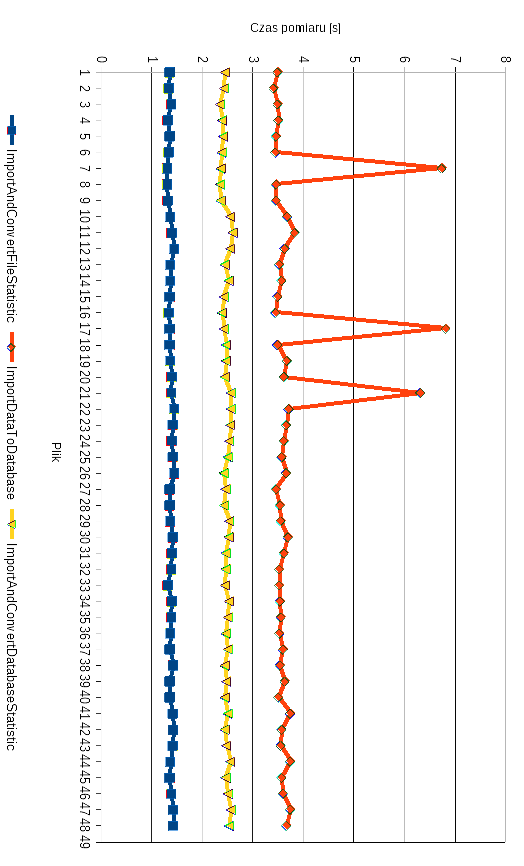
\includegraphics[width=\linewidth]{resources/statystyka_pomiaru.png}
    \caption{Przedstawienie wyników pomiaru czasu importu danych do aplikacji}
    \label{fig:importdata}
\end{figure}
\newpage
\subsection{Dokładność algorytmów i porównanie punktów wynikowych}